\documentclass[11pt,letterpaper]{extarticle}
\usepackage[T1]{fontenc}
\usepackage[utf8]{inputenc}
\usepackage[default]{sourcesanspro}
\usepackage[letterpaper, left=0.7in, right=0.7in, top=0.75in, bottom=0.75in,
            headheight=15pt, headsep=0.2in, footskip=0.35in]{geometry}
\usepackage{xcolor}
\usepackage{tikz}
\usetikzlibrary{arrows.meta}
\usepackage{fancyhdr}
\usepackage{array}
\usepackage{tabularx}
\usepackage{enumitem}
\usepackage{titlesec}
\usepackage{amsmath}
\usepackage{lastpage}
\usepackage{needspace}

% ---------------------------------------------------------------- page style
\pagestyle{fancy}
\fancyhf{}
\fancyhead[L]{\small Week 3 / Shuffle machines / Adult guide}
\fancyfoot[L]{\small Bellingham Math Circle / Week 3 / F03-FAC-v5}
\fancyfoot[R]{\small \thepage}
\renewcommand{\headrulewidth}{0pt}
\renewcommand{\footrulewidth}{0pt}

\setlength{\parindent}{0pt}
\setlength{\parskip}{4pt}
\raggedright
\setlist{nosep, leftmargin=1.2em}
\titleformat{\section}{\large\bfseries}{\thesection}{0.5em}{}
\titlespacing*{\section}{0pt}{10pt}{3pt}
\titleformat{\subsection}{\normalsize\bfseries}{}{0pt}{}
\titlespacing*{\subsection}{0pt}{8pt}{2pt}
\renewcommand{\arraystretch}{1.15}

% ---------------------------------------------------------------- colours (as on the student mats)
\definecolor{cg}{HTML}{3FAE4A}
\definecolor{cb}{HTML}{2F6FD6}
\definecolor{cr}{HTML}{D8343C}
\definecolor{cy}{HTML}{F5C518}
\definecolor{cp}{HTML}{7D46A8}
\definecolor{ck}{HTML}{F07AB4}
\definecolor{shade}{gray}{0.93}

% a row of cubes, slot 1 on the left: \crow{g,b,r}
\newcommand{\crow}[1]{\tikz[baseline=-0.05em]{\foreach \c [count=\i] in {#1}
  \filldraw[fill=c\c, draw=black, line width=0.3pt] ({(\i-1)*0.9em},-0.05em) rectangle +(0.75em,0.75em);}}
% "after turn k"
\newcommand{\tn}[1]{\hspace{0.7em}{\footnotesize #1:}\hspace{0.15em}}
% arrow list from targets: \arrs{3,1,2} -> 1->3, 2->1, 3->2
\newcommand{\ar}{\ensuremath{\to}}
\newcommand{\arrs}[1]{\foreach \t [count=\i] in {#1}{\ifnum\i>1, \fi\i\ar\t}}
% small mat drawing: \minimat{3,1,2} or \minimat[g,b,r]{3,1,2} (colour tabs = home pictures)
\newcommand{\minimat}[2][]{\begin{tikzpicture}[x=1.3pt,y=1.3pt,baseline=0pt]
  \foreach \t [count=\i] in {#2} {
    \draw[line width=0.5pt] ({(\i-1)*12},24) rectangle +(10,10);
    \draw[line width=0.5pt] ({(\i-1)*12},0) rectangle +(10,10);
    \draw[line width=0.75pt,-{Stealth[length=3.4pt,width=3.4pt]}] ({(\i-1)*12+5},24) -- ({(\t-1)*12+5},10);
    \fill ({(\i-1)*12+5},24) circle (0.9pt);}
  \if\relax\detokenize{#1}\relax\else
  \foreach \c [count=\i] in {#1} \filldraw[fill=c\c, draw=black, line width=0.3pt] ({(\i-1)*12+2},36) rectangle +(6,4);\fi
\end{tikzpicture}}
% a mini mat with a caption under it, and a centred row of them
\newcommand{\mmc}[3][]{\begin{tabular}[b]{@{}c@{}}\minimat[#1]{#2}\\[-2pt]{\footnotesize #3}\end{tabular}}
\newcommand{\mmrow}[1]{\par\vspace{2pt}{\centering #1\par}\vspace{2pt}}

\newcommand{\core}{\textsf{\small\colorbox{shade}{core}}}
\newcommand{\further}{\textsf{\small further}}
% problem entry: \prob{1}{core}{page 1}{what the children do}
\newcommand{\prob}[4]{\par\needspace{6\baselineskip}\vspace{5pt}\textbf{Problem #1} \,#2\, \textit{(#3)}\hspace{0.5em}#4\par}
\newcommand{\ans}{\textbf{Answer.} }
\newcommand{\hints}{\textbf{Hints.} }
\newcommand{\watch}{\textbf{Watch for.} }

% written by check_answers.py from the drawn machines in ../src/fig; do not edit
\newcommand{\KoneA}{\tn{1}\crow{b,r,g}\tn{2}\crow{r,g,b}\tn{3}\crow{g,b,r}}
\newcommand{\KoneB}{\tn{1}\crow{g,r,b}\tn{2}\crow{g,b,r}}
\newcommand{\KtwoA}{\tn{1}\crow{y,r,g,b}\tn{2}\crow{b,g,y,r}\tn{3}\crow{r,y,b,g}\tn{4}\crow{g,b,r,y}}
\newcommand{\KtwoB}{\tn{1}\crow{r,y,g,b}\tn{2}\crow{g,b,r,y}}
\newcommand{\KthreeA}{\tn{1}\crow{y,g,r,b}\tn{2}\crow{b,y,r,g}\tn{3}\crow{g,b,r,y}}
\newcommand{\KthreeB}{\tn{1}\crow{r,p,g,b,y}\tn{2}\crow{g,y,r,p,b}\tn{3}\crow{r,b,g,y,p}\tn{4}\crow{g,p,r,b,y}\tn{5}\crow{r,y,g,p,b}\tn{6}\crow{g,b,r,y,p}}
\newcommand{\KsixRow}{\crow{r,y,b,g}}
\newcommand{\MfourRowA}{\crow{r,g,y,b}}
\newcommand{\MfourRowB}{\crow{b,p,y,r,g}}
\newcommand{\MsixOneAB}{\crow{b,r,g,y}}
\newcommand{\MsixOneBA}{\crow{r,g,b,y}}
\newcommand{\MsixTwoAB}{\crow{r,y,g,b}}
\newcommand{\MsixTwoBA}{\crow{r,y,g,b}}
\newcommand{\LaunchRows}{\tn{1}\crow{b,g,y,p,r}\tn{2}\crow{g,b,p,r,y}\tn{3}\crow{b,g,r,y,p}\tn{4}\crow{g,b,y,p,r}\tn{5}\crow{b,g,p,r,y}\tn{6}\crow{g,b,r,y,p}}


\begin{document}

{\Large\bfseries Shuffle machines: adult guide}\par
\vspace{2pt}
{\small For the student packets F03-K-v5 (K--1), F03-M-v5 (grades 2--3) and F03-U-v5 (grades 4--5). Slots are numbered 1, 2, 3, \dots\ from the left. Every answer here was recomputed by \texttt{check\_answers.py} from the machines drawn on the student pages.}

% ============================================================================================
\section{The idea of the week}

A shuffle machine is a mat with a top row of slots, a bottom row, and one arrow from each top slot to a bottom slot, with exactly one arrow arriving at each bottom slot. One turn: every cube goes down its own arrow, then the whole bottom row slides straight up. Run a machine over and over and every cube comes back home, under the picture of its colour. Following the arrows from any slot leads back to that slot, so the slots split into loops, and a cube in a loop of 3 is home every 3 turns. The whole row is home when all the loops are home together, so loops of 2 and 3 take 6 turns: more turns than cubes. Machines can be undone (reverse every arrow) and combined (run one, then the other), and a perfect card shuffle is a machine too.

\begin{tabularx}{\linewidth}{@{}>{\bfseries}p{0.55in}X@{}}
K--1 & Every child runs machines with cubes, moving all the cubes down before sliding the row up, and keeps a tally of turns. A good hour reaches Problem 4: each child draws a machine for 2 or 3 turns and the partner checks it with cubes. Someone says that the 5-cube machine took 6 turns, or that a cube on a straight arrow is home after every turn.\\
2--3 & Children trace loops on the page and predict before running. A good hour reaches Problem 4, and a child can say why loops of 2 and 3 take 6 turns (``the pair is home at 2, 4, 6; the three are home at 3, 6'').\\
4--5 & Children predict without cubes, list every return time for 5 slots with a reason (all the ways to split 5 slots into loops), and do the 8-card shuffle by hand and draw it as a machine. A good hour reaches Problem 5 with explanations; the quickest child is on Problems 6--9.\\
\end{tabularx}

% ============================================================================================
\section{Materials and preparation}

\subsection{Cubes, not pattern blocks}
The mat slots are about 1.2 inches square. That is too small for most pattern blocks: a trapezoid is 2 inches long, a hexagon 2 inches across, a blue rhombus about 1.7 inches long. The pictures above the slots are only labels. Use snap cubes or other small objects in the colours of the pictures, and a cube goes \emph{home} under the picture of its colour: green under the green triangle (slot 1), blue under the blue rhombus (slot 2), red under the red trapezoid (slot 3), yellow under the yellow hexagon (slot 4), purple under the purple chevron (slot 5), pink under the pink triangle (slot 6). Pink appears only on the 6-slot mats of grades 2--3 Problem 2; if you have no pink cube, any small pink object that fits a slot will do.

\vspace{2pt}
\begin{tabularx}{\linewidth}{@{}lXl@{}}
\textbf{Table} & \textbf{Cubes} & \textbf{Total} \\ \hline
K--1 (4 children) & one set of 5 per child (green, blue, red, yellow, purple), plus 1 spare set & 25: 5 of each colour\\
2--3 (4 children) & one set of 6 per child (the same 5 and pink), plus 1 spare set & 30: 5 of each colour\\
4--5 (3 children) & one set of 5 per child, plus 1 spare set & 20: 4 of each colour\\ \hline
\end{tabularx}
All tables together: 75 cubes, 14 each of green, blue, red, yellow and purple, and 5 pink. The pages say ``blocks''; the cubes are the blocks.

Put each set in its own cup. The launch borrows the K--1 spare set. Each table also needs pencils, coloured pencils (at least three colours per child at 2--3, for colouring loops), one small whiteboard and marker per child (fallback games), and scrap paper. The 4--5 table gets the two decks of playing cards: before the session put one suit A, 2, \dots, 10, J, Q in order on top of each deck, so children can take the top 4, 6, 8, 10 or 12 cards; keep the decks complete for Problem 10.

\subsection{Printing}
Print single-sided on US Letter, \textbf{in colour}, at \textbf{100\% (``Actual size'', not ``Fit to page'')}: the slots must stay 1.2 inches and the pictures must show their colours.

\begin{tabularx}{\linewidth}{@{}lccX@{}}
\textbf{Packet} & \textbf{Pages} & \textbf{Copies} & \textbf{How it is handed out}\\ \hline
K--1, F03-K-v5 & 10 & 6 & 4 children, the adult, 1 spare. One page at a time. On pages 1--3 and 7 a pair shares one sheet (one child moves, the other tallies). On pages 4--6 and 8 each child has a sheet. Pages 9 and 10: one partner takes each.\\
2--3, F03-M-v5 & 11 & 6 & 4 children, the adult, 1 spare. One page at a time, one per child.\\
4--5, F03-U-v5 & 8 & 5 & 3 children, the adult, 1 spare. One page at a time, one per child, the referee included.\\
Test mats & 1 & 4 & Extra copies of K--1 page 9 (a blank 5-slot mat with pictures): 2 for the 2--3 table, 2 for the 4--5 table, to run machines drawn on the small mats.\\
This guide & \pageref*{LastPage} & 3 & One per adult.\\
\end{tabularx}

\subsection{Set up before the children arrive}
\textbf{Floor map for the launch.} Five chairs in a row, about 3 feet apart, facing the group. Tape a sheet of coloured paper to the front of each chair, where it shows while a child sits, left to right: green, blue, red, yellow, purple (the order of the mats). With masking tape, lay one arrow per chair on the floor in front of the chairs, as in the drawing: each arrow starts at the front of its chair, runs out into its own lane (about 1 foot or 2 feet from the chairs), and ends at the front of another chair. Mark each start with a short crossbar (like the dot on the mats) and each end with a V of tape. The arrows do not cross.

\begin{center}
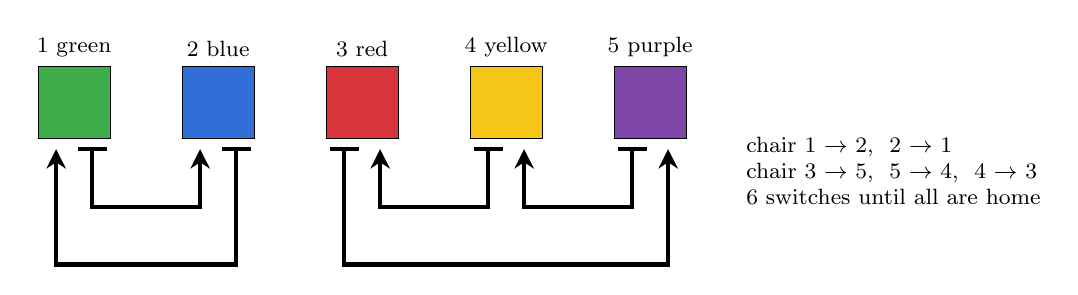
\begin{tikzpicture}[x=0.36in,y=0.36in]
  \foreach \c/\n [count=\i] in {cg/green,cb/blue,cr/red,cy/yellow,cp/purple} {
    \filldraw[fill=\c, draw=black] ({2*(\i-1)-0.5},0.15) rectangle ({2*(\i-1)+0.5},1.15);
    \node[font=\footnotesize, above] at ({2*(\i-1)},1.15) {\i\ \n};}
  \foreach \a/\d/\b in {0.25/0.8/1.75, 2.25/1.6/-0.25, 3.75/1.6/8.25, 5.75/0.8/4.25, 7.75/0.8/6.25} {
    \draw[line width=1.6pt, -{Stealth[length=7pt,width=7pt]}] (\a,0) -- (\a,-\d) -- (\b,-\d) -- (\b,0);
    \draw[line width=1.6pt] (\a-0.2,0) -- (\a+0.2,0);}
  \node[font=\footnotesize, anchor=west, align=left] at (9.2,-0.3) {chair 1 \ar\ 2, \ 2 \ar\ 1\\ chair 3 \ar\ 5, \ 5 \ar\ 4, \ 4 \ar\ 3\\ 6 switches until all are home};
\end{tikzpicture}
\end{center}

\textbf{At each table:} one cup of cubes per child, the packet pages in order face down, coloured pencils and whiteboards within reach. Nothing needs cutting.

\subsection{Test with the real materials (each adult, 10 minutes, the day before)}
\begin{enumerate}
\item Put real cubes on a printed K--1 page 1 and grades 2--3 page 2 (a 6-slot mat; its slots are 1.15 inches). Each cube should sit inside one slot with the arrows still visible. Check that each cube's colour clearly matches its picture, especially blue against purple, and the pink.
\item Run K--1 Problem 3's 5-slot machine (page 3, bottom) once. It takes 6 turns; the rows are in Section 4.
\item 4--5 table: do one 8-card perfect shuffle with the cards in a row and check that you get A, 5, 2, 6, 3, 7, 4, 8.
\end{enumerate}

% ============================================================================================
\section{The hour}

\begin{tabularx}{\linewidth}{@{}lX@{}}
0:00--0:05 & Running around.\\
0:05--0:08 & Whole-group launch at the chairs, then at one mat.\\
0:08--0:48 & Work at the three tables, in pairs.\\
0:48--0:55 & Sharing: one question.\\
0:55--1:00 & Cubes back in cups, pages collected.\\
\end{tabularx}

\subsection{Launch (the organizer leads; about 3 minutes)}
\textbf{At the chairs.}
\begin{enumerate}
\item Pick five children to sit, one per chair (K--1 children first). Hand each one the cube of their chair's colour. Say: ``This cube shows your home chair.''
\item Say: ``Each chair has one arrow on the floor that starts at it. When I say \emph{switch}, everyone walks along the arrow that starts at your chair and sits in the chair at its end. Everyone moves at the same time. Everybody else, count the switches.''
\item Say ``switch''. After each switch ask: ``Is everyone home?'' After 2 switches green and blue are home: ``Green and blue are home. Are we done?'' Keep going. After 3, red, yellow and purple are home, but green and blue are not. After 6 everyone is home: ``Six switches, and only five chairs.''
\end{enumerate}
Who sits in chairs 1--5 after each switch:\\
\LaunchRows

\textbf{At one mat} (the spare K--1 page 1, top machine, on a table where everyone can see).
\begin{enumerate}[resume]
\item Say: ``The pictures are labels. The green cube lives under the green triangle.'' Put the green, blue and red cubes in the top slots under their pictures.
\item One child shows a legal turn. Say: ``Move every cube down its own arrow.'' The child moves each cube from its top slot to the bottom slot at the end of its arrow (one cube at a time is fine: the bottom row starts empty). Then: ``Now slide the whole bottom row straight up.'' The child pushes the row up into the top slots. Say: ``That is one turn. Every cube moves every turn, even on a straight arrow.''
\end{enumerate}
Not legal: moving some cubes and not others; moving a cube from a top slot straight to another top slot; sliding the row sideways.

\subsection{Pairs}
\begin{tabularx}{\linewidth}{@{}>{\bfseries}p{0.55in}X@{}}
K--1 & Two pairs, each a kindergartner with a first grader. On running pages one child is the \emph{mover} (moves the cubes, slides the row) and the other the \emph{counter} (makes a tally after each turn, says when every cube is home); swap at each machine. On drawing pages each child draws and the partner checks the drawing with cubes.\\
2--3 & Two pairs. One child runs the cubes, the other checks each turn and records; swap at each machine. In Problem 6 one partner runs A then B while the other runs B then A, and they compare rows.\\
4--5 & A pair and a referee. The referee checks that every turn or shuffle is legal, keeps the count, and settles disagreements by running it again. The referee changes at each new problem. In Problem 5 the referee repeats the shuffle with the second deck.\\
\end{tabularx}

\subsection{When attention runs out}
\begin{tabularx}{\linewidth}{@{}>{\bfseries}p{0.55in}X@{}}
K--1 & \emph{Human machine.} Put four sticky notes (green, blue, red, yellow) on the floor beside the table; each child stands on one. Draw four arrows on a whiteboard (two rows of four boxes). On ``switch'' everyone walks to the colour their arrow points to; count switches until everyone is back on their own colour. Children take turns drawing the arrows.\\
2--3 & \emph{Predict and run.} One partner draws a 5-slot machine on a whiteboard. The other says how many turns it will take before any cube moves, then they run it with cubes. A correct prediction scores a point; swap.\\
4--5 & \emph{Slowest machine.} The two players each draw an 8-slot machine on a whiteboard without looking at each other's. The referee finds the loops and the number of turns; more turns wins. Then 9 slots, then 10 (this leads into Problem 9).\\
\end{tabularx}

\subsection{Sharing (0:48)}
Ask the whole group one question: \textbf{``Show us a machine that takes more turns than it has slots. Why does it take so long?''} Each table has one: K--1 Problem 3 (5 slots, 6 turns), 2--3 Problem 1 (5 slots, 6 turns) or 8 (7 slots, 12 turns), 4--5 Problem 2 (7 slots, 10 turns) or 4.

% ============================================================================================
\section{Table by table}

\subsection{K--1 (parent volunteer)}
Read each problem aloud. Problems 1--4 are the core of the hour; 5--8 are for children who get further. If a child is struggling, stay on Problems 1--3 (running machines is the main thing), do only the 2-turn mat in Problem 4, and skip Problems 6 and 7. The coloured rows show the cubes in slots 1, 2, 3, \dots\ after each turn.

\prob{1}{\core}{page 1}{Run two 3-cube machines; make a tally for each turn.}
\ans Top machine: 3 turns. \KoneA. Bottom machine: 2 turns. \KoneB. On the bottom machine green has a straight arrow: it goes down and back up and is home after every turn; blue and red swap.\\
\hints (1) Point at the blue cube: ``Which arrow starts under it? Where does it end?'' (2) Move the cubes down one at a time, then push the whole row up together. (3) After each turn: ``Is every cube under its own picture?''\\
\watch Stopping when one cube is home; forgetting to slide the row up; moving a cube straight across the top row.

\prob{2}{\core}{page 2}{The same with four cubes, on two machines.}
\ans Top: 4 turns. \KtwoA. Bottom: 2 turns. \KtwoB. Green and red swap, and blue and yellow swap.\\
\hints (1) Before running: ``Will this take more turns than page 1, or fewer?'' (2) Follow one cube with a finger. (3) As in Problem 1.

\prob{3}{\core}{page 3}{The same on a 4-slot and a 5-slot machine.}
\ans Top: 3 turns. \KthreeA. Red has a straight arrow and never leaves; the other three go round.\\
Bottom (five cubes): 6 turns.\\
\KthreeB\\
Green and red swap and are home after 2 and 4 turns; blue, yellow and purple are home after 3; all five only after 6. Children say ``five cubes but six turns'' or ``green and red were home but we had to keep going''.\\
\hints (1) ``Which cubes are home after 2 turns? Keep going.'' (2) ``Is every cube home, or only some?'' (3) Keep making tallies even when some cubes are home.

\prob{4}{\core}{pages 4--5}{Draw arrows so the cubes come home in 2, 3 and 4 turns; the partner checks with cubes.}
\ans Many drawings are right; the cubes decide. \emph{2 turns:} two cubes swap and the others go straight down (9 machines, counting two swaps at once). \emph{3 turns:} three cubes go round and one goes straight down (8 machines). \emph{4 turns:} all four go round (6 machines). Examples:
\mmrow{\mmc[g,b,r,y]{2,1,3,4}{2 turns}\qquad \mmc[g,b,r,y]{2,3,1,4}{3 turns}\qquad \mmc[g,b,r,y]{2,3,4,1}{4 turns}}
\watch Two arrows into one bottom slot, or a bottom slot with no arrow. The cubes show it (two cubes in one slot, or an empty slot); ask the child to fix the arrows.\\
\hints (1) ``Which machine on pages 1--2 took 2 turns? Can you copy its idea?'' (2) For 2 turns: ``Make two cubes swap places.'' (3) For 4 turns: ``Make every cube go one slot to the right, and the last one go back to the first slot.''

\prob{5}{\further}{page 6}{Can only one cube end up in a different slot?}
\ans No. With the cubes: if the green cube goes to the blue slot, the blue cube cannot stay there, because two cubes cannot share a slot, so blue moves too. On the drawing: the bottom slot that green's arrow points to already has an arrow coming in. The fewest cubes that can change slots is two (a swap).\\
\hints (1) ``Draw it, then run it with the cubes. What happens in the bottom row?'' (2) ``Where does the cube that was in that slot go?'' (3) ``What is the fewest cubes that can change places?''

\prob{6}{\further}{page 7}{One turn on the first machine, move the row to the second mat in the same order, then draw arrows so one more turn sends every cube home.}
\ans After one turn the row is \KsixRow. The only answer: \arrs{3,4,2,1} (red to slot 3, yellow to 4, blue to 2, green to 1). It is the first machine with every arrow reversed:
\mmrow{\mmc[g,b,r,y]{4,3,1,2}{first machine}\qquad \mmc[g,b,r,y]{3,4,2,1}{answer on the second mat}}
\watch Putting the cubes back under their pictures before drawing; then straight arrows look right. Keep the order red, yellow, blue, green.\\
\hints (1) ``Where does the red cube live? Draw an arrow from red to its home.'' (2) One cube at a time. (3) ``On the first machine green went from slot 1 to slot 4. Which way must it go now?''

\prob{7}{\further}{page 8}{Draw all the machines with 3 slots. How many are there?}
\ans 6 (nine mats are printed, so three stay empty). Nobody moves (1 turn); two cubes swap and one goes straight (3 machines, 2 turns); all three go round, one way or the other (2 machines, 3 turns):
\mmrow{\mmc[g,b,r]{1,2,3}{1 turn}\qquad \mmc[g,b,r]{2,1,3}{2 turns}\quad \mmc[g,b,r]{1,3,2}{2 turns}\quad \mmc[g,b,r]{3,2,1}{2 turns}\qquad \mmc[g,b,r]{2,3,1}{3 turns}\quad \mmc[g,b,r]{3,1,2}{3 turns}}
Why no more, as a child can say it: ``Green's arrow can go to 3 places. Then blue's has 2 places left, and red's gets the last one.'' Two drawings that send every cube to the same place are the same machine, even if the lines bend differently.\\
\hints (1) ``Is there a machine where nobody moves?'' (2) ``Where can green's arrow go? Make one machine for each place.'' (3) Put two drawings side by side: ``Do these send the cubes to the same places?''

\prob{8}{\further}{pages 9--10}{Each partner draws a different 5-slot machine that takes 6 turns.}
\ans 20 machines with 5 slots take 6 turns (19 besides Problem 3's). Every one has two cubes that swap and three that go round. Examples: \arrs{2,1,4,5,3}; \ \arrs{3,4,5,2,1}.\\
\hints (1) ``On Problem 3's machine, which cubes swapped and which went round?'' (2) ``Choose two different cubes to swap.'' (3) ``Now make the other three go round.''

% --------------------------------------------------------------------------------------------
\subsection{Grades 2--3 (mathematician)}
Problems 1--4 are the core; 5--8 are further. If a child is struggling: in Problem 2 do the 5-slot machine and one 6-slot machine, in Problem 3 stop at 5 turns, and skip Problems 5 and 7. Loops are written in cycle notation: (1\,4\,3) means slot 1\ar4\ar3\ar1. The small mats (Problems 3, 5, 7, 8) are too small for cubes: run a drawn machine on a spare K--1 page 9 test mat, or trace it with a finger.

\prob{1}{\core}{page 1}{Each block's first return, and the first time all are home.}
\ans 4 slots, \arrs{4,2,1,3}, loops (1\,4\,3)(2): green 3, blue 1, red 3, yellow 3; all blocks 3.\\
5 slots, \arrs{3,5,4,1,2}, loops (1\,3\,4)(2\,5): green 3, blue 2, red 3, yellow 3, purple 2; all blocks 6.\\
\hints (1) ``Follow only the green cube. Where is it after each turn?'' (2) ``Blue is home after 2 turns. When else?'' (3) ``When are blue and green home at the same time?''

\prob{2}{\core}{pages 2--3}{Colour the loops, predict, then run.}
\ans
\begin{tabular}[t]{@{}llll@{}}
Mat & Machine & Loops & Turns\\ \hline
5 slots, p.\,2 & \arrs{2,5,1,4,3} & (1\,2\,5\,3)(4) & 4\\
6 slots, p.\,2 & \arrs{4,3,6,1,2,5} & (1\,4)(2\,3\,6\,5) & 4, not 8\\
6 slots, p.\,3 top & \arrs{4,1,6,2,3,5} & (1\,4\,2)(3\,6\,5) & 3, not 6\\
6 slots, p.\,3 bottom & \arrs{5,6,3,1,4,2} & (1\,5\,4)(2\,6)(3) & 6\\
\end{tabular}\\[2pt]
To trace a loop: start at a top slot, follow its arrow down, go straight up to the top slot above, follow that arrow, and stop when you are back. A straight arrow is a loop of 1.\\
\hints (1) ``Put your finger on top slot 1. Follow the arrow, jump straight up, follow again. When are you back?'' (2) ``Colour the slots you touched, then start again from a slot with no colour.'' (3) ``A loop of 2 is home after 2, 4, 6 turns; a loop of 4 after 4, 8. When are both home?''

\prob{3}{\core}{page 4}{A 5-slot machine for each number of turns from 1 to 6.}
\ans 1: all straight. 2: \arrs{2,1,3,4,5}. 3: \arrs{2,3,1,4,5}. 4: \arrs{2,3,4,1,5}. 5: \arrs{2,3,4,5,1}. 6: \arrs{2,1,4,5,3} (a swap and a loop of 3).\\
\hints (1) ``How many turns does a loop of 3 take? A loop of 5?'' (2) ``Which machine in Problem 1 took more turns than it has slots?'' (3) For 6: ``Split the 5 slots into two loops.''

\prob{4}{\core}{pages 5--6}{One turn, move the row to the empty mat, draw the machine that sends every cube home.}
\ans 4 slots, \arrs{2,4,1,3}: after one turn \MfourRowA; answer \arrs{3,1,4,2}.
5 slots, \arrs{5,1,4,3,2}: after one turn \MfourRowB; answer \arrs{2,5,4,3,1}.
Each answer is the only one, and is the machine with every arrow reversed; it has the same loops and the same number of turns (4 and 6).\\
\watch Cubes put back under their pictures on the empty mat.\\
\hints (1) ``Where does the red cube live? Draw that arrow first.'' (2) ``Which arrow on the first machine brought red here?'' (3) ``Compare your arrows with the first machine's arrows.''

\prob{5}{\further}{page 7}{Four 5-slot machines that undo themselves; how to tell from the loops.}
\ans There are 26: all straight (1), one swap and the rest straight (10), two swaps and one straight (15). A machine undoes itself exactly when every loop has 1 or 2 slots. With cubes: in a swap each cube goes over and back in two turns; in a loop of 3 or more, after two turns a cube is two steps along its loop, not home.\\
\hints (1) ``Run your Problem 4 machine twice. Is every cube home?'' (2) ``Try a machine where two cubes swap.'' (3) ``Run a loop of 3 for two turns. Where is each cube?''

\prob{6}{\further}{pages 8--9}{A then B, and B then A, for two pairs.}
\ans Pair 1 (p.\,8): A swaps slots 1 and 2; B swaps 2 and 3. A then B gives \MsixOneAB, B then A gives \MsixOneBA: different. Pair 2 (p.\,9): A swaps 1 and 3; B swaps 2 and 4. Both orders give \MsixTwoAB: the same. Why, with cubes: in pair 2, A only moves the cubes in slots 1 and 3 and B only the cubes in slots 2 and 4, so each does its own job whatever the other did. In pair 1 both use slot 2: B moves whichever cube A has just put there.\\
\hints (1) ``Which slots does A change? Which does B change?'' (2) ``In A then B, which cube does B move?'' (3) ``Can you make a new pair where the order matters? One where it does not?''

\prob{7}{\further}{page 10}{Which numbers of turns are possible with 6 slots? Explain.}
\ans Exactly 1, 2, 3, 4, 5, 6, the same as with 5 slots. Why: the loop sizes add up to 6, and there are 11 ways to split 6:
6\ar6; 5+1\ar5; 4+2\ar4; 4+1+1\ar4; 3+3\ar3; 3+2+1\ar6; 3+1+1+1\ar3; 2+2+2\ar2; 2+2+1+1\ar2; 2+1+1+1+1\ar2; 1+1+1+1+1+1\ar1. None gives more than 6. Machines: each Problem 3 machine with a straight arrow in slot 6.\\
\hints (1) ``List the ways to split 6 slots into loops, biggest loop first.'' (2) ``Which split could give 7 or more?'' (3) ``Why do loops of 2 and 4 take only 4 turns?''

\prob{8}{\further}{page 11}{A 7-slot machine with more than 10 turns; the most possible.}
\ans Only loops of 3 and 4 do it: 12 turns, for example \arrs{2,3,1,5,6,7,4}. The most is 12. Why: the splits of 7 give 7\ar7, 6+1\ar6, 5+2\ar10, 5+1+1\ar5, 4+3\ar12, 4+2+1\ar4, 3+3+1\ar3, 3+2+2\ar6, 3+2+1+1\ar6, and the other six splits give 4 or less.\\
\hints (1) ``A single loop of 7 takes 7. Can two loops do better?'' (2) ``Loops of 5 and 2 take 10. Can you beat 10?'' (3) ``List all the ways to split 7.''

% --------------------------------------------------------------------------------------------
\subsection{Grades 4--5 (organizer)}
Problems 1--5 are the core; 6--10 are further. If a child is struggling: in Problem 2 do only the 6- and 7-slot machines, and in Problem 5 use only 4, 6 and 8 cards. Composition: ``A then B'' sends slot $i$ to $B(A(i))$.

\prob{1}{\core}{page 1}{Each block's first return, and all blocks.}
\ans \arrs{3,2,5,1,4}, loops (1\,3\,5\,4)(2): 4, 1, 4, 4, 4; all 4.\\
\arrs{5,4,1,2,3}, loops (1\,5\,3)(2\,4): 3, 2, 3, 2, 3; all 6.\\
\hints (1) ``Follow only the green cube. Where is it after each turn?'' (2) ``Which turns is blue home after? And green?''

\prob{2}{\core}{page 2}{Turns for six machines, without cubes.}
\ans\enspace{\small\begin{tabular}[t]{@{}llll@{\qquad}llll@{}}
top left & 6 slots & (1\,3\,5)(2\,6\,4) & 3 & top right & 6 slots & (1\,5)(2\,3\,6)(4) & 6\\
middle left & 7 slots & (1\,4\,7\,2\,5)(3\,6) & 10 & middle right & 7 slots & (1\,4\,2\,7\,3\,5\,6) & 7\\
bottom left & 8 slots & (1\,3\,2\,5\,7\,6)(4\,8) & 6 & bottom right & 8 slots & (1\,3\,6\,8)(2\,5\,7\,4) & 4\\
\end{tabular}}\\
\hints (1) ``Follow slot 1 until you are back. Which slots did you visit?'' (2) ``When are a loop of 2 and a loop of 6 both home?''

\prob{3}{\core}{page 3}{All possible turns for 5 slots, with a reason.}
\ans 1, 2, 3, 4, 5, 6. The loop sizes add up to 5, and the seven splits give 5\ar5, 4+1\ar4, 3+2\ar6, 3+1+1\ar3, 2+2+1\ar2, 2+1+1+1\ar2, 1+1+1+1+1\ar1. A child's explanation: ``Every machine is some loops. Here is every way to make loops from 5 slots, biggest loop first, and what each one takes.''\\
\hints (1) ``What loops can 5 slots hold?'' (2) ``How do you know your list of splits is complete?''

\prob{4}{\core}{page 4}{Slowest machines with 6 and 7 slots.}
\ans 6 slots: 6 turns, by one loop of 6 or by loops 3+2+1. 7 slots: 12 turns, only by loops 4+3. Why none is slower: the 11 splits of 6 and the 15 splits of 7 (listed under grades 2--3, Problems 7 and 8).\\
\hints (1) ``Which machine on page 2 has 7 slots and the most turns? Can you beat it?'' (2) ``List the ways to split 7 slots into loops.'' (3) ``When are a loop of 3 and a loop of 4 both home?''

\prob{5}{\core}{page 5}{Perfect shuffles of 4--12 cards; the 8-card shuffle as a machine.}
\ans 4 cards: 2. 6: 4. 8: 3. 10: 6. 12: 10. The 8-card machine is \arrs{1,3,5,7,2,4,6,8}, with loops (2\,3\,5)(4\,7\,6) and the top and bottom cards fixed, so 3 shuffles. A card in position $k$ goes to $2k-1$ in the top half and $2k-8$ in the bottom half.
To shuffle in a row: split the row into a top-half row and a bottom-half row under it, then take cards alternately, top row first, into a new row.\\
\watch Dealing alternately onto a pile, which reverses the deck (8, 4, 7, 3, 6, 2, 5, A); the printed example catches it.\\
\hints (1) ``Check your first 8-card shuffle against A, 5, 2, 6, 3, 7, 4, 8.'' (2) ``Follow the card that starts in position 2.'' (3) ``Draw the machine and find its loops.''

\prob{6}{\further}{page 6}{Draw A then B and B then A for three pairs.}
\ans\enspace{\small\begin{tabular}[t]{@{}lllll@{}}
 & A & B & A then B & B then A\\ \hline
pair 1 & \arrs{2,1,3,4} & \arrs{1,3,2,4} & \arrs{3,1,2,4} & \arrs{2,3,1,4}\\
pair 2 & \arrs{2,1,3,4} & \arrs{1,2,4,3} & \arrs{2,1,4,3} & \arrs{2,1,4,3}\\
pair 3 & \arrs{2,3,1,4} & \arrs{1,3,4,2} & \arrs{3,4,1,2} & \arrs{2,1,4,3}\\
\end{tabular}}\\[2pt]
Pair 1: two swaps sharing slot 2 give loops of 3 going opposite ways. Pair 2: swaps on separate slots agree. Pair 3: both orders are two swaps, but different ones.\\
\hints (1) ``Run A then B with cubes on a test mat and draw where each cube ends up.'' (2) ``Follow slot 1: where does A send it? Where does B send that slot?'' (3) ``Which slots do A and B both use?''

\prob{7}{\further}{page 7}{Undo A, B and A then B; the rule for undoing A then B.}
\ans\enspace{\small\begin{tabular}[t]{@{}lll@{}}
 & pair 1 (top) & pair 2 (bottom)\\ \hline
A & \arrs{2,3,1,4} & \arrs{2,1,3,4}\\
B & \arrs{1,4,2,3} & \arrs{1,3,4,2}\\
A then B & \arrs{4,2,1,3} & \arrs{3,1,4,2}\\
undoes A & \arrs{3,1,2,4} & \arrs{2,1,3,4} (A itself)\\
undoes B & \arrs{1,3,4,2} & \arrs{1,4,2,3}\\
undoes (A then B) & \arrs{3,2,4,1} & \arrs{2,4,1,3}\\
\end{tabular}}\\[2pt]
Rule: undo (A then B) = undo B, then undo A. With cubes: the last thing done was B, so undo it first; that leaves the row as A left it, and undoing A finishes. (Socks, then shoes; the shoes come off first.) The other order fails for both pairs. Reversing every arrow of A then B gives the same machine.\\
\hints (1) ``Run A then B with cubes. Which machine brings them all home in one turn?'' (2) ``Which machine did you run last? Undo that one first.'' (3) ``Try undo A then undo B, and undo B then undo A. Which one works?''

\prob{8}{\further}{page 8}{Two different 4-slot machines, each moving all four blocks, with A then B = B then A.}
\ans Of the 9 machines that move all four blocks there are 12 such pairs: any two of the three double swaps (3 pairs, e.g. \arrs{2,1,4,3} with \arrs{3,4,1,2}); a loop of 4 and the same loop reversed (3 pairs, e.g. \arrs{2,3,4,1} with \arrs{4,1,2,3}); a loop of 4 and that loop run twice (6 pairs, e.g. \arrs{2,3,4,1} with \arrs{3,4,1,2}).\\
\hints (1) ``Try two machines whose loops have the same sizes.'' (2) ``What about a machine and the same machine run twice?''

\prob{9}{\further}{page 8}{Most turns for 1 to 10 slots; is one more slot always slower?}
\ans 1, 2, 3, 4, 6, 6, 12, 15, 20, 30. Record loops: 5 slots 3+2; 6 slots 6 or 3+2+1; 7 slots 4+3; 8 slots 5+3; 9 slots 5+4; 10 slots 5+3+2. No: 6 slots cannot beat 5 slots (both 6). One more slot never does worse (add a cube that stays put), and from 1 to 10 slots the step from 5 to 6 is the only one with no gain.\\
\hints (1) ``For 8 slots, which two loops could beat 12?'' (2) ``Is the record for 6 slots bigger than for 5?'' (3) ``Why can one more slot never make the record smaller?''

\prob{10}{\further}{page 8}{Perfect shuffles for 52 cards.}
\ans 8. A card in position $k$ goes to $2k-1$ if $k\le 26$ and to $2k-52$ if $k\ge 27$. The card in position 2 visits 2, 3, 5, 9, 17, 33, 14, 27 and is back after 8 shuffles. The whole 52-card machine has six loops of 8, one loop of 2 (positions 18 and 35), and the top and bottom cards stay, so every card is home after 8 shuffles and not before. Counting positions from 0, position $i$ goes to $2i \bmod 51$, and $2^8 = 256 = 5\cdot 51+1$.\\
\hints (1) ``Where does the card in position 2 go? Position 3?'' (2) ``Find a rule for where a card in the top half goes.'' (3) ``Follow one card until it comes back. Is every card back by then?''

% ============================================================================================
\section{The mathematics behind the week}

\textbf{Machines are permutations.} A machine on $n$ slots is a bijection $\sigma$ of $\{1,\dots,n\}$: one arrow out of each top slot and one into each bottom slot. One turn sends the block in slot $i$ to slot $\sigma(i)$. There are $n!$ machines (6 with 3 slots).

\textbf{Loops are cycles.} Follow $i, \sigma(i), \sigma^2(i), \dots$. Some value repeats; if $\sigma^a(i)=\sigma^b(i)$ with $0<a<b$ and $a$ least, injectivity gives $\sigma^{a-1}(i)=\sigma^{b-1}(i)$, against the choice of $a$. So the first repeat is $i$ itself, and the slots split into disjoint cycles. No machine moves exactly one block: if $\sigma(i)=j\ne i$, then $\sigma(j)\ne j$ because $j$ already has an arrow in.

\textbf{Return time is a least common multiple.} A block in a cycle of length $k$ is home exactly after multiples of $k$ turns, so the whole row first returns after $\operatorname{lcm}$ of the cycle lengths (the order of $\sigma$). The possible return times on $n$ slots are the lcms of the partitions of $n$: $\{1,\dots,6\}$ for 5 and for 6 slots; 1--7, 10 and 12 for 7. The largest is Landau's function $g(n)$: 1, 2, 3, 4, 6, 6, 12, 15, 20, 30 for $n=1,\dots,10$. It never decreases (add a fixed point) but can stay level, and $\log g(n)\sim\sqrt{n\log n}$.

\textbf{Undoing and combining.} The inverse reverses every arrow and has the same cycle type, hence the same order. ``A then B'' is $B\circ A$; in general $B\circ A\ne A\circ B$ (two swaps sharing a slot give opposite 3-cycles), but machines moving disjoint sets of slots commute. Since $(B\circ A)^{-1}=A^{-1}\circ B^{-1}$, the machine that undoes ``A then B'' is ``undo B, then undo A''. A machine undoes itself (an involution) exactly when all its cycles have length 1 or 2; on 5 slots there are $1+10+15=26$.

\textbf{Perfect shuffles.} Number positions $0,\dots,2m-1$. The out-shuffle sends position $i$ to $2i \bmod (2m-1)$ and fixes the last card, so its order is the multiplicative order of 2 modulo $2m-1$: 4, 6, 8, 10, 12 and 52 cards give 2, 4, 3, 6, 10 and 8 (for 52, $2^8 = 256 \equiv 1 \pmod{51}$). The in-shuffle (bottom half's card first) sends $i$ to $2i+1 \bmod (2m+1)$; for 52 cards it needs 52 shuffles, since 2 has order 52 modulo 53.

\textbf{Where it goes next.} Two machines with the same cycle type are the same machine with the slots relabelled (conjugacy). Every machine is a product of swaps, and the parity of their number is fixed (the sign), which explains why half the positions of the 15 puzzle are unreachable. Elmsley's trick: to move the top card to position $k$ (counting from 0), write $k$ in binary and, reading from the left, do an in-shuffle for each 1 and an out-shuffle for each 0. Diaconis, Graham and Kantor (1983) found the whole group generated by the two perfect shuffles. Sources: Judson, \emph{Abstract Algebra}, Ch.~5; Diaconis, Graham and Kantor, ``The mathematics of perfect shuffles''.

% ============================================================================================
\clearpage
\section{What to write down after the session}

Each adult fills in their row the same evening. Photograph one page per table that shows a drawing or a claim worth keeping. For each claim, write whether the children \textbf{tried} it (ran one case), \textbf{guessed} it, \textbf{checked} it in some cases, or \textbf{explained} it.

Claims to listen for: ``more slots always means more turns'' (false: 5 and 6 slots both give at most 6); ``a machine with 5 slots takes 5 turns''; ``loops of 2 and 4 take 8 turns''; ``you can't move just one cube''; ``there are 6 machines with 3 slots''; ``A then B is the same as B then A''.

\vspace{4pt}
\renewcommand{\arraystretch}{1.3}
\begin{tabularx}{\linewidth}{|>{\bfseries}p{0.42in}|>{\raggedright\arraybackslash}p{1.2in}|>{\raggedright\arraybackslash}X|>{\raggedright\arraybackslash}X|>{\raggedright\arraybackslash}p{1.0in}|}
\hline
Table & Problems reached (circle) & What children tried and said & Drawing or claim worth keeping & Tried, guessed, checked or explained\\ \hline
K--1 & 1 2 3 4 5 6 7 8 & & & \\[1.7in] \hline
2--3 & 1 2 3 4 5 6 7 8 & & & \\[1.7in] \hline
4--5 & 1 2 3 4 5 6 7 8 9 10 & & & \\[1.7in] \hline
\end{tabularx}

\end{document}
